% =====================================================================
%  chapter03_logistics.tex — לוגיסטיקה ואופרציות
% =====================================================================
\chapter{לוגיסטיקה ואופרציות}
\chaptersubtitle{איך לארגן את התיק לטיול של חמש דקות שנגמר בשעה}

\section{האנטומיה של ״אני רק יוצא לשנייה״}
כל בעל כלב מכיר את זה: יצאתם ״רק להוריד אותו״, בכפכפים ובלי טלפון, ואז הכלב מצא חבר, השכן
מצא נושא לשיחה והשמש החליטה לצאת במלוא העוצמה. הטיול של חמש דקות נמשך שעה, ואתם בלי מים ובלי
שקית שנייה. הפתרון הוא לא לצאת פחות, אלא להתארגן פעם אחת ולהפסיק לחשוב על זה.

\section{הערכה הבסיסית}
\begin{tcolorbox}[enhanced,colback=white,colframe=navy,arc=3mm,boxrule=0.8pt,
   title={\sffamily\bfseries\paw[white]\enspace רשימת ציוד קבועה ליד הדלת},colbacktitle=navy,
   left=8pt,right=8pt]
\begin{itemize}[label={\color{sagedark}$\square$}]
  \item \textbf{רצועה וקולר או רתמה תקינים}, עם תג ובו מספר טלפון עדכני. בישראל החוק מחייב גם
        סימון בשבב אלקטרוני, רישוי וחיסון נגד כלבת \cite{il-doglaw2002}.
  \item \textbf{שקיות לאיסוף צואה}: תמיד אחת יותר ממה שנראה לכם הגיוני.
  \item \textbf{מים וכלי שתייה מתקפל}, במיוחד בימים חמים ובמסלולים בלי ברזייה \cite{avma-warm}.
  \item \textbf{חטיפים קטנים} לתגמול על התנהגות רגועה (ראו פרק 1).
  \item \textbf{טלפון טעון} ומספר הווטרינר ומוקד החירום הקרוב שמורים בו מראש.
  \item \textbf{לפי מזג האוויר}: מעיל לכלב קטן או קצר-פרווה בחורף, ופנס או אפוד מחזיר-אור בלילה.
\end{itemize}
\end{tcolorbox}

\begin{fieldbox}
קנו שני עותקים מכל דבר קטן: שקיות, כלי שתייה וחטיפים. סט אחד גר קבוע בתיק הטיולים, והסט השני
במגירה ליד הדלת. ככה לא ״שואלים״ ציוד מתיק לתיק, ולא נשארים בלי.
\end{fieldbox}

\section{המתמטיקה של יום עירוני}
כדי לתכנן יום עמוס, כדאי לדעת כמה זמן הטיולים לוקחים בפועל. מספר הטיולים ביום יסומן באות $n$,
ומשך הטיול מספר $i$ (בדקות) יסומן $t_i$. זמן הטיול היומי הכולל הוא:

\begin{equation}
  T_{\text{daily}} \;=\; \sum_{i=1}^{n} t_i
  \label{eq:daily}
\end{equation}

\textbf{דוגמה היפותטית:} נניח ארבעה טיולים: 20 דקות בבוקר, 15 בצהריים, 35 בערב ועשר דקות לפני השינה.
אז
\[
  T_{\text{daily}} = 20 + 15 + 35 + 10 = 80 \ \text{min}.
\]
כלומר, כשעה ועשרים דקות ביום, ועוד ״מקדם הפתעות״ של מפגשים, ריחות ושכנים. בפועל, כדאי לשריין
ביומן קצת יותר ממה שהנוסחה אומרת.

\begin{figure}[h]
  \centering
  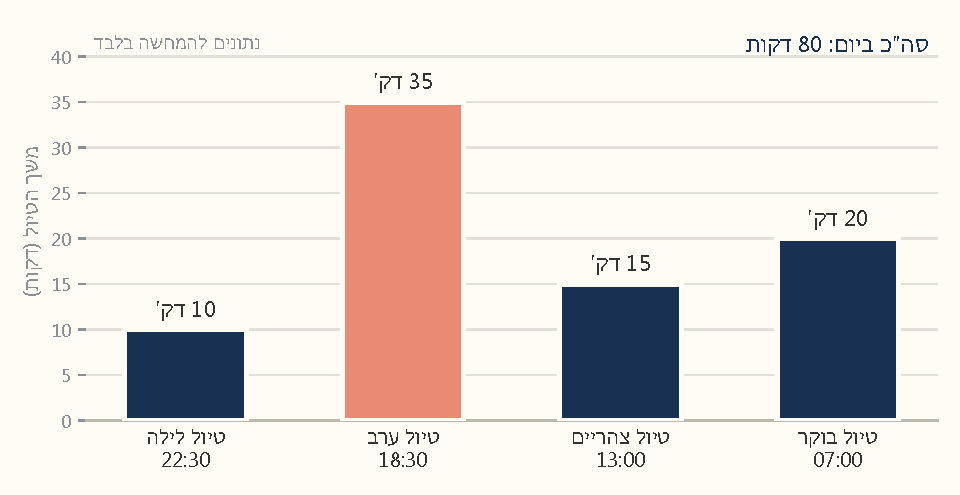
\includegraphics[width=0.82\linewidth]{activity_graph.pdf}
  \caption{חלוקת זמן הטיולים לאורך יום עירוני לדוגמה. הגרף נוצר בקוד \en{Python} (\en{matplotlib})
  מהנתונים של הדוגמה שלמעלה. \textbf{הנתונים להמחשה בלבד} ואינם המלצה וטרינרית.}
  \label{fig:graph}
\end{figure}

\begin{knowbox}
אין ״מספר דקות נכון״ אחד לכל הכלבים. גור, כלב צעיר ואנרגטי, כלב מבוגר וכלב עם בעיה רפואית צריכים
דברים שונים מאוד, וגם מזג האוויר משנה את התמונה. את הכמות והעצימות המתאימות לכלב שלכם כדאי לקבוע
יחד עם הווטרינר.
\end{knowbox}

\section{לתכנן סביב עבודה, חיים ובלת״מים}
\begin{itemize}
  \item \textbf{עוגנים קבועים:} טיול בוקר וטיול ערב בשעות דומות בכל יום יוצרים שגרה צפויה.
  \item \textbf{תוכנית ב׳ לצהריים:} שכנה, בן משפחה או מוליך כלבים, ומספר טלפון שמור מראש.
  \item \textbf{״מקדם עיכוב״:} הוסיפו ליומן כרבע שעה רזרבה סביב כל טיול. מה שלא נוצל הוא בונוס.
  \item \textbf{ימים חמים:} מקדימים את הבוקר, מאחרים את הערב ומקצרים את הצהריים
        (ראו פרק 2 ומקור \cite{avma-warm}).
\end{itemize}

\section{שבוע לדוגמה}
השגרה היומית מתחברת לשבוע. הטבלה הבאה היא דוגמה היפותטית למשק בית עם שני אנשים עובדים וכלב
בוגר ובריא. היא לא מתכון: המטרה היא להראות איך מחלקים אחריות כך שאף טיול לא ״נופל בין הכיסאות״.

\begin{table}[h]
\centering
\caption{שבוע לדוגמה: מי מוציא את הכלב ומתי (נתונים להמחשה בלבד)}
\label{tab:week}
\renewcommand{\arraystretch}{1.3}
\small
\begin{tabularx}{\linewidth}{>{\sffamily\bfseries\color{navy}}p{1.9cm} X X X}
\toprule
{\sffamily\bfseries יום} & {\sffamily\bfseries בוקר} & {\sffamily\bfseries צהריים} & {\sffamily\bfseries ערב ולילה} \\
\midrule
ראשון–רביעי & א׳: טיול רגיל & שכנה או מוליך כלבים & ב׳: טיול ארוך, ואחר כך יציאה קצרה \\
\rowcolor{sage!10}
חמישי & ב׳: טיול רגיל & א׳ עובד מהבית & טיול משותף לגינת הכלבים \\
שישי & טיול ארוך בפארק & יציאה קצרה & א׳: טיול רגיל \\
\rowcolor{sage!10}
שבת & טיול רגוע עם הרבה ריחרוח & מנוחה, משחקי חיפוש בבית & ב׳: טיול רגיל \\
\bottomrule
\end{tabularx}
\end{table}

\begin{fieldbox}
תלו את הטבלה על המקרר או שתפו אותה ביומן משותף. כשמשהו משתנה, מעדכנים במקום אחד, וכל מי
שמעורב בטיפול בכלב רואה את אותה תמונה.
\end{fieldbox}

\section{תיק חירום קטן}
מלבד תיק הטיולים היומי, כדאי להכין בבית תיק קטן שמוכן ליום שבו משהו משתבש: נסיעה דחופה
לווטרינר, הפסקת חשמל ארוכה או פינוי זמני מהבית.
\begin{itemize}
  \item צילום של פנקס החיסונים ומספר השבב, גם בטלפון וגם על נייר.
  \item רצועה וקולר רזרביים, עם תג זיהוי מעודכן.
  \item מזון ומים לכמה ימים, וכלי האכלה מתקפל.
  \item תרופות קבועות, אם יש כאלה, לפי הנחיות הווטרינר.
  \item ערכת עזרה ראשונה לבעלי חיים, שאת תכולתה כדאי לתאם עם הווטרינר.
  \item מגבת, שקיות ותמונה עדכנית של הכלב, למקרה שיאבד.
\end{itemize}

\begin{mistakebox}
לצאת ״על הדרך״ לסידורים עם כלב שלא רגיל לכך: תור בדואר, חנות צפופה ומדרכה רותחת. לכלב זה
עומס חושי, ולכם זה תור שנמשך כפליים. עדיף טיול קצר וממוקד, ואת הסידורים לעשות אחר כך.
\end{mistakebox}
